\chapter{Coordinates}
\index{coordinates|hyperbf}

%-----------------------------------------------------------------------------
\section{Local Reference Coordinates}
\label{s:local.coords}

%-----------------------------------------------------------------------------
\subsection{Local Reference Orbit}
\label{s:ref}
\index{reference orbit|hyperbf}

\begin{figure}[!b]
  \centering
  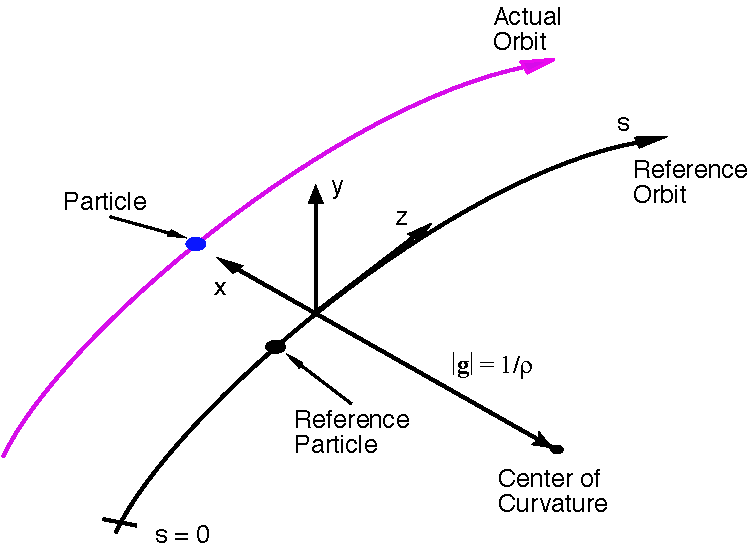
\includegraphics[height=8.4cm]{local-coords.pdf}
  \caption[The local Reference System.]
{The local reference coordinate system. By construction, a particle's
$z$ coordinate is zero.  This is not to be confused with the phase
space $z$ coordinate (\sref{s:phase.space}). The curvature vector
$\bfg$ lies in the $x$-$y$ plane and has a magnitude of $1/\rho$ where
$\rho$ is the bending radius. The $z$-axis will normally be parallel
to the $s$-axis but for \vn{reversed} elements it will be antiparallel.
}
  \label{f:local.coords}
\end{figure}

The \vn{local reference orbit} is the curved path used to define a
coordinate system for describing a particle's position as shown in
\fig{f:local.coords}. The reference orbit is also used for orientating
lattice elements in space. At a given time $t$, a particle's position
can be described by a point on the reference orbit a distance $s$
relative to the reference orbit's zero position plus a transverse
offset. This point on the reference orbit is used as the origin of the
local $(x, y, z)$ coordinate system with the $z$--axis tangent to the
reference orbit. The $z$--axis will generally be pointing in the
direction of increasing $s$ but, as discussed in detail below, will
point counter to $s$ for elements that are \vn{reversed}. The $x$ and
$y$--axes are perpendicular to the reference orbit. As will be shown
later, If the lattice has no vertical bends, the $y$--axis is in the
vertical direction and the $x$--axis is in the horizontal
plane. Notice that, by construction, the particle is always at $z =
0$. The coordinate system so constructed is called the \vn{``local
coordinate system''} or sometimes the \vn{``laboratory coordinate
system''} when there is need to distinguish it from the \vn{``element
coordinate system''} (\sref{s:ele.coords}) which is attached to
the physical element.

There is a separate reference orbit for each branch
(\sref{s:branch.def}) of a lattice. When there are multiple branches,
the reference orbit of a branch must not depend upon the configuration
of branches later on in the array of branches in the lattice. As a
consequence, the reference orbits of the branches can be calculated
one at a time starting with the first branch.

\index{x_offset}\index{y_offset}
\index{x_pitch}\index{y_pitch}\index{wiggler}
Notice that, in a \vn{wiggler}, the reference orbit, which is a
straight line, does {\em not} correspond to the orbit that any actual
particle could travel. Typically the physical element is
centered with respect to the reference curve. However, by specifying offsets, 
pitches or a tilt (See \sref{s:offset}), the physical element may be
arbitrarily shifted with respect to its reference curve. Shifting a
physical magnet with respect to its reference curve generally means
that the reference curve does {\em not} correspond to the orbit that
any actual particle could travel.

Do not confuse this reference orbit (which defines the local
coordinate system) with the reference orbit about which the transfer
maps are calculated (\sref{s:twiss}). The former is fixed by the
lattice while the latter can be any arbitrary orbit.

%-----------------------------------------------------------------------------
\subsection{Reference Orbit Construction: Upstream, Downstream, Entrance, and Exit Element Ends}
\label{s:ref.construct}
\index{reference orbit!construction}
\index{upstream element end}\index{downstream element end}
\index{entrance element end}\index{exit element end}

%--------------------------------------

  \begin{figure}[tb]
  \centering
  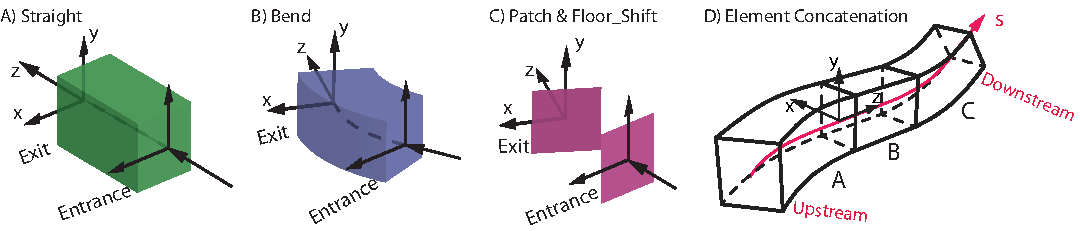
\includegraphics{element-coord-frame.pdf}
\caption[Element LEGO blocks.]{Element reference frame LEGO
blocks. Shown are the blocks along with the entrance and exit
reference frames. The physical element may be displaced in the local
coordinate frame using offsets, tilt, and pitches. A) For straight
line elements the two frames are colinear. B) For bends elements, the
two frames are rotated with respect to each other. C) For \vn{patch}
and \vn{floor_shift} elements the exit frame may be arbitrarily
positioned with respect to the entrance.}
  \label{f:ele.coord.frame}
  \end{figure}

%--------------------------------------

\begin{figure}[tb]
  \centering
  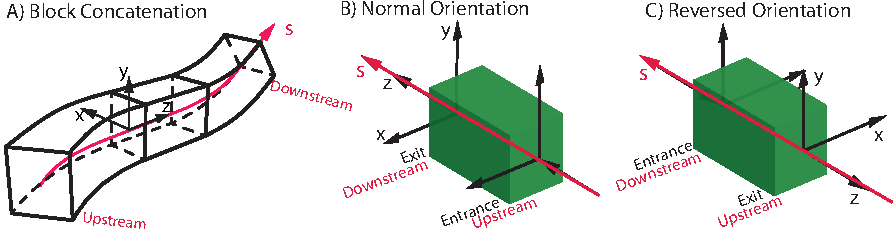
\includegraphics{element-stream.pdf}
  \caption[Element LEGO block concatenation.]{
Element LEGO block concatenation. A) The reference orbit is
constructed by concatenating the LEGO blocks together. B) For normal
(non-reversed) elements the $z$-axis is parallel with the $s$-axis. C)
For \vn{reversed} elements the $z$-axis is antiparallel with the
$s$-axis. By definition, the ``entrance'' and ``exit'' ends of an
element are fixed relative to the element (relative to the $z$-axis)
while the ``upstream'' and ``downstream'' ends are fixed relative to
the $s$-axis.}
  \label{f:stream}
\end{figure}

%--------------------------------------

\index{sbend}\index{rbend}
\index{crystal}\index{mirror}\index{entrance_end}
\index{exit_end}\index{patch}\index{floor_shift}
Another way of thinking about the reference orbit is to imagine that
each element has assigned to it a local coordinate reference frame
assigned to it in the shape of a LEGO block\footnote{Thanks to Dan
Abell for this analogy.} as shown in \fig{f:ele.coord.frame}.  Every
block has an ``\vn{entrance}'' and an ``\vn{exit}'' reference frame.
For most types of elements, the LEGO block for the element is
``straight'' as shown in \fig{f:ele.coord.frame}A. That is, the
reference curve through the block is a straight line segment and the
length of the block is the length of the element. For a \vn{bend}
(\sref{s:bend}), the reference curve through the block is a segment of
a circular arc as shown in \fig{f:ele.coord.frame}B. With a zero
\vn{ref_tilt}, the rotation axis between the entrance and exit frames of a
bend is the $y$-axis (\sref{s:global}). For \vn{patch}
(\sref{s:patch}), and \vn{floor_shift} (\sref{s:floor.ele}) elements,
the exit face can can arbitrarily oriented with respect to the
entrance end. In this case, the reference orbit between the entrance
and exit faces is not defined.

\index{root branch}
Assuming for the moment that there are no \vn{fiducial} elements
present, the construction of the reference orbit starts at the
beginning element of a branch. If the branch is a \vn{root} branch
(\sref{s:lattice.def}), The orientation of the beginning element can
be set via the appropriate positioning statements
(\sref{s:beginning}). If the branch is not a \vn{root} branch, the
position of the beginning element is determined by the position of the
\vn{fork} or \vn{photon_fork} element from which the branch forks
from.

Once the beginning element in a branch is positioned, succeeding
element LEGO blocks are concatenated together as illustrated in
\fig{f:stream}A. When a block is joined, the end of the block that is
mated to the previous block is called the ``\vn{upstream}'' end and
the other end which will be mated to the following block is called the
``\vn{downstream}'' end.  Normally, the \vn{entrance} end of a block
is used as the \vn{upstream} end the \vn{exit} end is used as the
\vn{downstream} end as shown in \fig{f:stream}B. However, for
\vn{reversed} elements (\sref{s:ele.reverse}), the \vn{upstream} end
is the \vn{exit} end of the block and vice versa. To put it another
way, the \vn{entrance} and \vn{exit} end of the blocks reference the
physical element. Thus, for example, the \vn{e1} edge of a bend
(\sref{s:bend}) is always at the \vn{entrance} face and the \vn{e2} is
always at the \vn{exit}face. Also the field of a wiggler is
(\sref{s:wiggler}) is referenced to $z = 0$ which is at the
\vn{entrance} end. The \vn{upstream} and \vn{downstream} ends, on the
other hand, are referenced to the reference orbit and the
\vn{downstream} end always is at a larger $s$ position relative to the
\vn{upstream} end.

In all cases, when a LEGO block is joined to the previous block, the
coordinate system at the mating end of the block (the \vn{upstream}
end) will be aligned with the mating end of the previous block (the
\vn{downstream} end). The situation where one of the blocks is
reversed and the other one not, and neither is a \vn{patch} nor
\vn{floor_shift} element, does not make physical sense since a
particle which is moving downstream, when it comes to the face joining
the blocks will have to magically reverse direction in order to travel
through the next block. Thus, to have normal and reversed elements in
a branch, \vn{reflection} \vn{patches} must be used in between.
Whether it makes physical sense to put a \vn{patch} element next to
another element is more complicated. This depends upon whether the
other element is reversed or not and whether the \vn{patch} is
reversed, whether the \vn{patch} is \vn{reflecting}, and the sign of
\vn{z_offset} for the \vn{patch}. The basic criterion is that a
particle leaving one block must enter the next. See
Section~\sref{s:ex.patch} for an example.

If there are \vn{fiducial} elements, the local reference frame is
constructed beginning at these elements.

%-----------------------------------------------------------------------------

\begin{figure}[tb]
  \centering
  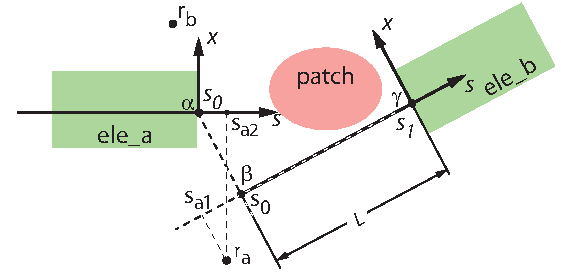
\includegraphics[width=5in]{patch-problem.pdf}
  \caption[The local reference coordinates in a \vn{patch} element.]
{The local reference coordinates in a \vn{patch} element. The
\vn{patch} element, shown schematically as an ellipse, is sandwiched
between elements \vn{ele_a} and \vn{ele_b}. \vn{L} is the length of
the \vn{patch}. In this example, the \vn{patch} has a finite
\vn{x_pitch}.}
  \label{f:patch.prob}
\end{figure}

%-----------------------------------------------------------------------------
%-----------------------------------------------------------------------------
\subsection{Patch Element Local Coordinates}
\label{s:patch.prob}
\index{patch}

Generally, if a particle is reasonably near the reference orbit, there
is a one-to-one mapping between the particle's position and $(x, y,
s)$ coordinates. A \vn{patch} (\sref{s:patch}) elements with non-zero
pitch breaks the one-to-one mapping. This is illustrated in
\fig{f:patch.prob}.  The \vn{patch} element, shown schematically as an
ellipse, is sandwiched between elements \vn{ele_a} and \vn{ele_b}. The
local coordinate system with origin at $\alpha$ are the coordinates at
the end of \vn{ele_a}. The coordinates at the end of the \vn{patch}
has its origin labeled $\gamma$. By convention, the length of the
patch \vn{L} is taken to be the longitudinal distance from $\alpha$ to
$\gamma$ with the \vn{patch}'s exit coordinates defining the
longitudinal direction. The ``beginning'' point of the \vn{patch} on the
reference orbit a distance \vn{L} from point $\gamma$ is labeled
$\beta$ in the figure.

In the local $(x, y, s)$ coordinate system a particle at $\alpha$ will
have some value $s = s_0$. A particle at point $\beta$ will have the
same value $s = s_0$ and a particle at $\gamma$ will have $s = s_1 =
s_0 + L$. A particle at point $r_a$ in \fig{f:patch.prob} illustrates
the problem of assigning $(x, y, s)$ coordinates to a given
position. If the particle is considered to be within the region of
\vn{ele_a}, the particle's $s$ position will be $s_{a2}$ which is
greater than the value $s_0$ at the exit end of the element. This
contradicts the expectation that particles within \vn{ele_a} will have
$s \le s_0$.  If, on the other hand, the particle is considered to be
within the \vn{patch} region, the particle's $s$ position will be
$s_{a1}$ which is less than the value $s_0$ at the entrance to the
patch. This contradicts the expectation that a particles within the
\vn{patch} will have $s \ge s_0$.

To resolve this problem, \bmad considers a particle at position $r_a$
to be within the \vn{patch} region. This means that there is, in
theory, no lower limit to the $s$-position that a particle in the
\vn{patch} region can have. This also implies that there is a
discontinuity in the $s$-position of a particle crossing the exit face
of \vn{ele1}. Typically, when particles are translated from the exit
face of one element to the exit face of the next, this \vn{patch}
problem does not appear. It only appears when the track between faces
is considered.

Notice that a particle at position $r_b$ in \fig{f:patch.prob} can
simultaneously be considered to be in either \vn{ele_a} or the
\vn{patch}. While this creates an ambiguity it does not complicate
tracking.

%-----------------------------------------------------------------------------
\section{Global Coordinates}
\label{s:global}
\index{global coordinates|hyperbf}

The Cartesian \vn{global} coordinate system, also called the `floor''
coordinate system, is the coordinate system ``attached to the earth''
that is used to describe the local coordinate system. Following the
\mad\ convention, the \vn{global} coordinate axis are labeled $(X, Y,
Z)$. Conventionally, $Y$ is the ``vertical'' coordinate and $(X, Z)$
are the ``horizontal'' coordinates. To describe how the local
coordinate system is oriented within the global coordinate system,
each point on the $s$-axis of the local coordinate system is
characterized by its $(X, Y, Z)$ position and by three angles $\theta$,
$\phi$, and $\psi$ that describe the orientation of the local coordinate axes
as shown in \fig{f:global.coords}. These three angles are defined as
follows:
\begin{description}
\item[$\theta$ Azimuth angle:] Angle in the $(X, Z)$ plane 
between the $Z$--axis and the projection of the $z$--axis onto the
$(X, Z)$ plane. A positive angle of $\theta = \pi/2$ corresponds to the
projected $z$--axis pointing in the positive $X$ direction.
\item[$\phi$ Pitch (elevation) angle:] Angle between the $z$--axis 
and the $(X,Z)$ plane. A positive angle of $\phi = \pi/2$ corresponds to
the $z$--axis pointing in the positive $Y$ direction.
\item[$\psi$ Roll angle:] Angle of the $x$--axis with respect 
to the line formed by the
intersection of the $(X, Z)$ plane with the $(x, y)$ plane. A
positive $\psi$ forms a right--handed screw with the $z$--axis.
\end{description}

\begin{figure}[tb]
\centering
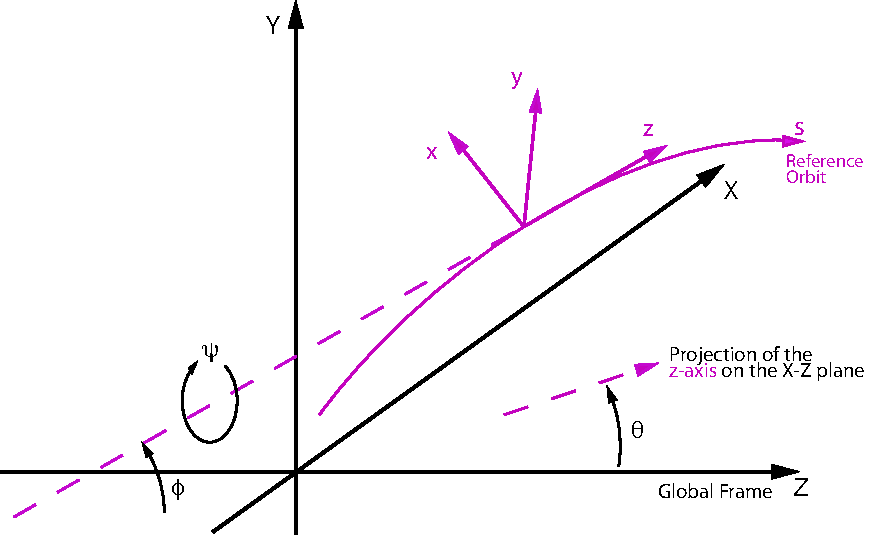
\includegraphics{global-coords.pdf}
\caption[The Global Coordinate System]{The Global Coordinate System.}
\label{f:global.coords}
\end{figure}

\index{beginning statement}
\index{reference orbit!origin in global coordinates}
\index{global coordinates!reference orbit origin}
By default, at $s = 0$, the reference orbit's origin coincides with
the $(X, Y, Z)$ origin and the $x$, $y$, and $z$ axes correspond to
the $X$, $Y$, and $Z$ axes respectively. $\theta$ decreases as one
follows the reference orbit when going through a horizontal bend with
a positive bending angle. This corresponds to $x$ pointing radially
outward. Without any vertical bends, the $Y$ and $y$ axes will
coincide, and $\phi$ and $\psi$ will both be zero. The \vn{beginning}
statement (\sref{s:beginning}) in a lattice file can be use to
override these defaults.

\index{MAD}
Following \mad, the global position of an element is characterized by
a vector $\bfV$ 
\Begineq
  \bfV = 
  \begin{pmatrix}
    X \\ Y \\ Z 
  \end{pmatrix}
\Endeq
The orientation of an element is described by a unitary matrix $\bfW$.
The column vectors of $\bfW$ are the unit vectors spanning the local
coordinate axes in the order $(x, y, z)$. $\bfW$ can be expressed in
terms of the angles $\theta$, $\phi$, and $\psi$ via the formula
\Begineq
  \bfW = \bfW_\Theta \, \bfW_\Phi \, \bfW_\Psi
  \label{wwww}
\Endeq
where
\Begineq
  \bfW_\Theta(\theta) = 
  \begin{pmatrix}
    \cos\theta  & 0 & \sin\theta \\
    0           & 1 & 0          \\
    -\sin\theta & 0 & \cos\theta 
  \end{pmatrix}, \quad
  \bfW_\Phi(\phi) = 
  \begin{pmatrix}
    1 & 0 & 0                \\
    0 & \cos\phi  & \sin\phi \\
    0 & -\sin\phi & \cos\phi 
  \end{pmatrix}, \quad
  \bfW_\Psi(\psi) = 
  \begin{pmatrix}
    \cos\psi & -\sin\psi & 0 \\
    \sin\psi &  \cos\psi & 0 \\
    0        &  0        & 1                
  \end{pmatrix}
  \label{wtt0t}
\Endeq

%-----------------------------------------------------------------------------
\subsection{Lattice Element Positioning}
\label{s:ele.pos}

\index{MAD}
\bmad, again following \mad, computes $\bfV$ and $\bfW$ by starting
at the first element of the lattice and iteratively using the
equations
\begin{align}
  \bfV_i &= \bfW_{i-1} \, \bfL_i + \bfV_{i-1}, 
    \label{vwlv} \\
  \bfW_i &= \bfW_{i-1} \, \bfS_i
    \label{wws}
\end{align}
$\bfL_i$ is the displacement vector for the $i$\Th element and matrix
$\bfS_i$ is the rotation of the local reference system of the exit
end with respect to the entrance end. For clarity, the subscript $i$ in 
the equations below will be dripped. For all elements whose
reference orbit through them is a straight line, the corresponding
$\bfL$ and $\bfS$ are
\Begineq
  \bfL = 
  \begin{pmatrix}
      0 \\ 0 \\ L
  \end{pmatrix},
  \quad
  \bfS = 
  \begin{pmatrix}
      1 & 0 & 0 \\ 
      0 & 1 & 0 \\
      0 & 0 & 1
  \end{pmatrix},
\Endeq
Where $L$ is the length of the element. 

%-----------------------------------------------------------------------

\begin{figure}
\centering 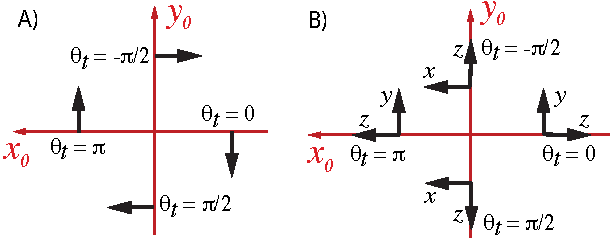
\includegraphics{tilt-bend.pdf} 
\caption[Orientation of a Bend.] 
  {
A) Rotation axes for four different \vn{ref_tilt} angles of $\theta_t$
= 0, $\pm \pi/2$, and $\pi$. $(x_0, y_0, z_0)$ are the local
coordinates at the entrance end of the bend with the $z_0$ axis being
directed into the page. Any rotation axis will be displaced by a
distance of the bend radius \vn{rho} from the origin. B) The $(x, y,
z)$ coordinates at the exit end of the bend for the same four
\vn{ref_tilt} angles. In this case the bend angle is taken to be
$\pi/2$.
  }
  \label{f:tilt.bend}
\end{figure}

%-----------------------------------------------------------------------

\index{rbend}\index{sbend}
\index{rho}\index{tilt}\index{angle}
For a \vn{bend}, the axis of rotation is dependent upon the bend's
\vn{ref_tilt} attribute as shown in \fig{f:tilt.bend}A. The axis of
rotation points in the negative $y_0$ direction for \vn{ref_tilt} = 0
and is offset by the bend radius \vn{rho}. Here $(x_0, y_0, z_0)$ are
the local coordinates at the entrance end of the bend with the $z_0$
axis being directed into the page in the figure.  For a non-zero
\vn{ref_tilt}, the rotation axis is itself rotated about the $z_0$
axis by the value of \vn{ref_tilt}. \fig{f:tilt.bend}B shows the
exit coordinates for four different values of \vn{ref_tilt} and for a
bend angle \vn{angle} of $\pi/2$.

For a bend, $\bfL$ and $\bfS$ are given by
\Begineq
  \bfL = \bfT \, \bftilde L, \quad
  \bfS = \bfT \, \bftilde S \, \bfT^{-1}
  \label{ltl}
\Endeq
where
\Begineq
  \bftilde L = 
  \begin{pmatrix}
    \rho (\cos\alpha_b - 1) \\ 0 \\ \rho \, \sin\alpha_b
  \end{pmatrix}, 
  \quad
  \bftilde S = 
  \begin{pmatrix}
    \cos\alpha_b & 0 & -\sin\alpha_b \\
    0          & 1 & 0           \\
    \sin\alpha_b & 0 & \cos\alpha_b
  \end{pmatrix},
  \quad
  \bfT = 
  \begin{pmatrix}
    \cos\theta_t & -\sin\theta_t & 0 \\
    \sin\theta_t &  \cos\theta_t & 0 \\
    0            &  0            & 1                
  \end{pmatrix}
  \label{lrca1}
\Endeq
with $\rho$ being the bend radius (\vn{rho}), $\alpha_b$ is the bend
\vn{angle} (\sref{s:bend}), and $\theta_t$ is the \vn{ref_tilt} angle
(\sref{s:offset}). Without a \vn{ref_tilt}, $\bfT$ is the unit matrix
resulting in $\bfL = \bftilde L$ and $\bfS = \bftilde
S$. Notice that for a bend in the horizontal $X-Z$ plane, a positive
bend \vn{angle} will result in a decreasing azimuth angle $\theta$.

The bend transformation (\Eq{ltl}) is so constructed that the
transformation is equivalent to rotating the local coordinate system
around an axis that is perpendicular to the plane of the bend. This
rotation axis is invariant under the bend transformation. For example,
for $\theta_t = 0$ (or $\pi$) the $y$-axis is the rotation axis and
the $y$-axis of the local coordinates before the bend will be parallel
to the $y$-axis of the local coordinates after the bend as shown in
\fig{f:tilt.bend}. That is, a lattice with only bends with
$\theta_t = 0$ or $\pi$ will lie in the horizontal plane (this
assuming that the $y$-axis starts out pointing along the $Y$-axis as
it does by default).  For $\theta_t = \pm\pi/2$, the bend axis is the
$x$-axis. A value of $\theta_t = +\pi/2$ represents a downward
pointing bend.

\begin{figure}
  \centering 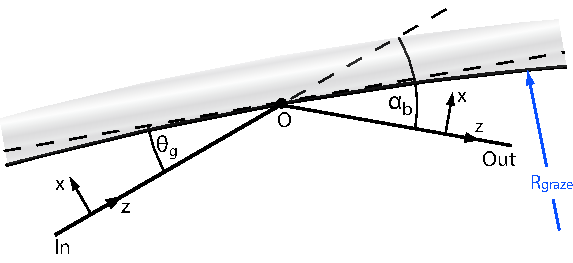
\includegraphics{mirror.pdf} 
\caption[Mirror and crystal geometry] {Mirror and crystal geometry.
The geometry shown here is appropriate for a \vn{ref_tilt} angle of
$\theta_t = 0$.  $\theta_g$ is the bend angle of the incoming
(entrance) ray, and $\alpha_b$ is the total bend
angle of the reference trajectory. A) Geometry for a mirror or a Bragg
crystal. Point $\calO$ is the origin of both the local coordinates
just before and just after the reflection/diffraction. B) Geometry for
a Laue crystal.  Point $\calO_{out}$ is the origin of the coordinates
just after diffraction is displaced from the origin $\calO_{in}$ just
before diffraction due to the finite thickness of the crystal. here
the bend angles are measured with respect to the line that is in
the plane of the entrance and exit coordinates and perpendicular to
the surface. For Laue diffraction, the user has the option of using
the undiffracted beam (shown in red) as the reference trajectory.
  }  
  \label{f:mirror}
\end{figure}

%-----------------------------------------------------------------------------
\subsection{Position Transformation When Transforming Coordinates}
\label{s:pos.trans}

A point $\bfR = (X, Y, Z)$ defined in the global coordinate system,
when expressed in the coordinate system defined by $(\bfV, \bfW)$ is
\Begineq
  \bfR_{VW} = \bfW^{-1} \left( \bfR - \bfV \right)
  \label{rwrv}
\Endeq
This is essentially the inverse of \Eq{vwlv}. That is, vectors
propagate inversely to the propagation of the coordinate system.

Using \Eq{rwrv} with \Eqs{vwlv}, and \eq{wws}, the transformation of a
particle's position $\bfr = (x,y,z)$ and momentum $\bfP = (P_x, P_y,
P_z)$ when the coordinate frame is transformed from frame
$(\bfV_{i-1}, \bfW_{i-1})$ to frame $(\bfV_i, \bfW_i)$ is
\begin{align}
  \bfr_i &= \bfS_i^{-1} \, \left( \bfr_{i-1} - \bfL_i \right), 
    \label{rwlr} \\
  \bfP_i &= \bfS_i^{-1} \, \bfP_{i-1}
    \label{pps}
\end{align}

Notice that since $\bfS$ (and $\bfW$) is the product of orthogonal
rotation matrices, $\bfS$ is itself orthogonal and its inverse is
just the transpose
\Begineq
  \bfS^{-1} = \bfS^T
\Endeq

%-----------------------------------------------------------------------------
\subsection{Crystal and Mirror Element Coordinate Transformation}
\label{s:mirror.coords}

\index{crystal}\index{mirror}\index{ref_tilt}
A \vn{crystal} element (\sref{s:mirror}) diffracts photons and a
\vn{mirror} element (\sref{s:mirror}) reflects them. For a crystal
setup for Bragg diffraction, and for a mirror, the reference orbit is
modeled as a zero length bend with $\bftilde L = (0, 0, 0)$, as shown
in \fig{f:mirror}A. Shown in the figure is the geometry
appropriate for a \vn{ref_tilt} angle of $\theta_t = 0$ (the rotation axis is
here the $y$-axis). Since the mirror or crystal element is modeled to
be of zero length, the origin points (marked $\calO$ in the figure)
of the entrance and exit local coordinates are the same. For Laue
diffraction, the only difference is that $\bftilde L$ is non-zero due
to the finite thickness of the crystal as shown in
\fig{f:mirror}B. This results in a separation between the
entrance coordinate origin $\calO_{in}$ and the exit coordinate
origin $\calO_{out}$.

In all cases, the total bending angle is
\begin{align}
  \alpha_b &= \text{bragg_angle_in} + \text{bragg_angle_out} &\text{! Crystal} \CRNO
  \alpha_b &= 2 \, \text{graze_angle}                        &\text{! Mirror}
  \label{agg}
\end{align}
With a mirror or Bragg diffraction, the bend angles are measured with
respect to the surface plane. With Laue diffraction the bend angles
are measured with respect to the line in the bend plane perpendicular
to the surface.

For Laue diffraction, the user has the option of using the
undiffracted beam (shown in red) as the reference trajectory.

The orientation of the exit coordinates (the local coordinates after
the reflection) are only affected by the element's \vn{ref_tilt} and
bend angle parameters and is independent of all other parameters such
as the radius of curvature of the surface, etc. The local $z$-axis of
the entrance coordinates along with the $z$-axis of the exit
coordinates define a plane which is called the element's \vn{bend
plane}.  For a mirror, the graze angle is a parameter supplied by the
user. For a crystal, the Bragg angles are calculated so that the
reference trajectory is in the middle of the Darwin curve. Calculation
of the Bragg angles for a crystal is given in
Section~\sref{ss:crystal.ref}.

%-----------------------------------------------------------------------------
\subsection{Element Misalignment and Origin Shift Transformation}
\label{s:patch.coords}

The \vn{Element Body} coordinates are the coordinate system attached
to an element. Without any misalignments (Here \vn{``misalignment''}
is {\em defined} to be any offset, pitch or tilt (\sref{s:offset}),
the laboratory and element body coordinates are the same. With
misalignments, the transformation is given by \Eqs{vwlv} and \eq{wws}
where 
\Begineq
  \bfL =  (\text{x_offset}, \, \text{y_offset}, \, \text{z_offset})
  \label{lxyz}
\Endeq
and the $\bfS$ matrix is defined by 
\Begineq
  \bfS = \bfW_\Theta \, \bfW_\Phi \, \bfW_\Psi
  \label{swww}
\Endeq
with
\Begineq
  \Theta = \text{x_pitch},  \qquad \Phi = \text{y_pitch},  \qquad \Psi = \text{tilt}
  \label{txppyp}
\Endeq
The form of \Eq{swww} was chosen to correspond to the form of \Eq{wwww}.

\index{patch}\index{floor_shift}
For \vn{patch} (\sref{s:patch}) and \vn{floor_shift} (\sref{s:floor.ele})
elements, the above equations are also used to calculate the the shift
in the reference coordinates from the entrance end to the exit end of
the element.

\index{rbend}\index{sbend}\index{roll}\index{tilt}
For \vn{rbend} and \vn{sbend} elements the above equations are modified
by using 
\Begineq
  \Psi = 0
\Endeq
This is used since, unlike other elements, the \vn{ref_tilt} attribute of
a bend affects the reference orbit (cf.~\Eq{ltl}). In the place of a
\vn{tilt}, the \vn{roll} attribute can be used (\sref{s:offset}). For
a \vn{roll}, the transformation at the entrance end to go from laboratory
coordinates to element coordinates is
\Begineq
  \bfL = 0, \qquad 
  \bfS = \bfW_\Theta(\text{-angle/2}) \, \bfW_\Psi(\text{roll}) \, \bfW_\Theta(\text{angle/2})
\Endeq
where \vn{angle} is the total bend angle.
The transformation back to the laboratory frame at the exit end of the bend is
\Begineq
  \bfL = 0, \qquad 
  \bfS = \bfW_\Theta(\text{angle/2}) \, \bfW_\Psi(\text{-roll}) \, \bfW_\Theta(\text{-angle/2})
\Endeq
Notice that these transformations are not inverses of one another.

\index{girder}\index{fiducial}
For \vn{fiducial} and \vn{girder} elements the above equations are
used to calculate the alignment of reference coordinates with respect
to ``\vn{origin}'' coordinates. In this case, the vector $\bfL$ is
constructed via
\Begineq
  \bfL = (\text{dx_origin}, \qquad \text{dy_origin}, \qquad \text{dz_origin})
\Endeq
And the attributes use to shift the reference coordinates orientation are:
\Begineq
  \Theta = \text{dtheta_origin}, \qquad \Phi = \text{dphi_origin}, \qquad \Psi = \text{dpsi_origin}
\Endeq

%-----------------------------------------------------------------------------
\subsection{Reflection Patch}
\label{s:reflect.patch}
\index{patch!reflection}

A \vn{Patch} (or a series of patches) that reflects the direction of
the \vn{z}-axis is called a \vn{reflection} \vn{patch}. By ``reflected
direction'' it is meant that the dot product $\Bf z_1 \cdot \Bf z_2$ is
negative where $\Bf z_1$ is the $z$-axis vector at the \vn{entrance}
face and $\Bf z_2$ is the $z$-axis vector at the \vn{exit} face. This
condition is equivalent to the condition on $\bfS$ in \Eq{swww} of
\Begineq
  S(3,3) < 0
  \label{s330}
\Endeq
Using \Eq{swww} gives after some simple algebra
\Begineq
  \cos(\text{x_pitch}) \, \cos(\text{y_pitch}) < 0
\Endeq
When there are a series of patches, The transformations of all the
patches are concatenated together to form an effective $\bfS$ which
can then be used with \Eq{s330}.

%-----------------------------------------------------------------------------
\section{Phase Space Coordinates}
\label{s:phase.coords}
\index{phase space coordinates|hyperbf}

%-----------------------------------------------------------------------------
\subsection{Reference Particle, Reference Energy, and Reference Time}
\label{s:ref.energy}
\index{reference particle|hyperbf}
\index{reference energy|hyperbf}
\index{reference time|hyperbf}

The \vn{reference energy} and \vn{reference time} are needed in
evaluating the phase space coordinates of charged particles
(\sref{s:phase.space}).  

All lattice elements, except for controller elements, have an
associated \vn{reference energy} energy.  The reference energy at the
start of a lattice's \vn{root branch} (\sref{s:branch.def}) is set in
the lattice file by setting the reference momentum (\vn{p0c}) or total
energy (\vn{E_tot}) using a \vn{parameter} (\sref{s:param}) or
\vn{beginning} (\sref{s:beginning}) statement. For other branches, the
energy at the start of the branch is set using the appropriate line
parameter (\sref{s:beginning}) statement.

\index{custom!reference energy}\index{em_field!reference energy}
\index{hybrid!reference energy}\index{lcavity!reference energy}
\index{patch!reference energy}
For most elements, the reference energy is the same as the reference
energy of the preceeding element. The following elements are
exceptions:
\begin{example}
  custom
  em_field
  hybrid
  lcavity
  patch
\end{example}
The reference energy of these elements is determined by tracking a
particle (the ``\vn{reference particle}'') through the element with the
particle starting on the reference orbit and whose energy is equal to
the reference energy.  The energy of the particle at the downstream
end is the reference energy of the element.

\index{wiggler!reference time}
Besides the reference energy, lattice elements have an associated
\vn{reference time} which is computed, for most elements, by the
time-of-flight of the \vn{reference particle} assuming that the
reference particle is following the reference orbit. Exceptions are
\vn{wiggler} elements which uses the time-of-flight of the actual
undulating trajectory. [Actually what is used in the computation of the
$z$ phase space coordinate (\Eq{zbctt}) is the sum of reference time
deltas of the elements that a particle has passed through. It is not
possible to assign a unique reference time to an element when particles
are recirculating through elements as in a storage ring.]

%-----------------------------------------------------------------------------
\subsection{Charged Particle Phase Space Coordinates}
\label{s:phase.space}
\index{phase space coordinates|hyperbf}

\begin{figure}
\centering 
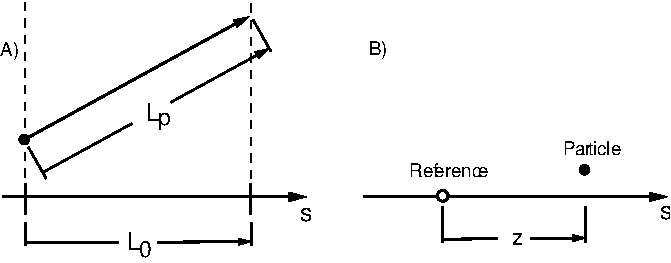
\includegraphics{canonical-z.pdf} 
\caption[Interpreting phase space $z$ at constant velocity.]
{Interpreting phase space $z$ at constant velocity: A) The change in $z$
going through an element of length $L_0$ is $L_0 - L_p$.  B) At
constant time, $z$ is the longitudinal distance between the reference
particle and the particle.}
\label{f:canonical.z}
\end{figure}

For charged particles (more correctly, for everything but photons
(\sref{s:photon.phase.space})), \bmad uses the phase space coordinates
\Begineq
  \Bf r(s) = (x, p_x, y, p_y, z, p_z)
\Endeq
The longitudinal position $s$ is the independent variable instead of
the time. $x$ and $y$, are the transverse coordinates of the particle
as shown in~\fig{f:local.coords}. Note that $x$ and $y$ are independent
of the position of the reference particle.

The phase space momenta $p_x$ and $p_y$ are normalized by the
reference (sometimes called the design) momentum $P_0$
\begin{align}
  p_x = &\frac{P_x}{P_0} \CRNO
  p_y = &\frac{P_y}{P_0}
  \label{ppp}
\end{align}
where $P_x$ and $P_y$ are respectively the $x$ and $y$ momentums.

\index{lcavity}\index{rfcavity}
The phase space $z$ coordinate is 
\begin{align}
  z(s) &= -\beta(s) \, c \, (t(s) - t_0(s)) \CRNO
    &\equiv - \beta(s) \, c \, \Delta t(s)
  \label{zbctt}
\end{align}
$t(s)$ is the time at which the particle is at position $s$, $t_0(s)$
is the time at which the reference particle is at position $s$, and
$\beta$ is $v/c$ with $v$ being the particle velocity (and not the
reference velocity). The reference particle is, by definition,
``synchronized'' with elements whose fields are oscillating and
therefore the actual fields a particle will see when traveling through
such an element will depend upon the particle's phase space $z$. For
example, the energy change of a particle traveling through an
\vn{lcavity} (\sref{s:lcav}) or \vn{rfcavity} (\sref{s:rfcav}) element
is $z$ dependent. Exception: With absolute time tracking
(\sref{s:rf.time}) fields are tied to the absolute time and not $z$.

If the particle's velocity is constant, and is
the same as the velocity of the reference particle (for example, at
high energy where $\beta = 1$ for all particles), then $\beta \, c \,
t$ is just the path length. In this case, the change in $z$ going
through an element is
\Begineq
  \Delta z = L_0 - L_p
\Endeq
where, as shown in \fig{f:canonical.z}A, $L_0$ is the path
length of the reference particle (which is just the length of the
element) and $L_p$ is the path length of the particle in traversing
the element.  Another way of interpreting phase space $z$ is that, at
constant $\beta$, and constant time, $z$ is the longitudinal distance
between the particle and the reference particle as shown in
\fig{f:canonical.z}B. with positive $z$ indicating that the
particle is ahead of the reference particle.

Do not confuse the phase space $z$ with the $z$ that is the particle's
longitudinal coordinate in the local reference frame as shown in
\fig{f:local.coords}. By construction, this latter $z$ is
always zero.

Notice that if a particle gets an instantaneous longitudinal kick so
that $\beta$ is discontinuous then, from \Eq{zbctt}, phase space $z$ is
discontinuous even though the particle itself does not move in
space. In general, from \Eq{zbctt}, The value of $z$ for a particle at
$s_2$ is related to the value of $z$ for the particle at $s_1$ by
\Begineq
  z_2 = \frac{\beta_2}{\beta_1} \, z_1 - 
  \beta_2 \, c \, (\Delta t_2 - \Delta t_1)
  \label{zbbzb}
\Endeq
$\Delta t_2 - \Delta t_1$ can be interpreted as the difference in
transit time, between the particle and the reference particle, in going
from $s_1$ to $s_2$.

The longitudinal phase space momentum $p_z$ is given by
\begin{equation}
  p_z = \frac{\Delta P}{P_0} \equiv \frac{P - P_0}{P_0}
  \label{ppppp}
\end{equation}
where $P$ is the momentum of the particle. For ultra--relativistic particles
$p_z$ can be approximated by
\begin{equation}
  p_z = \frac{\Delta E}{E_0}
\end{equation}
\index{lcavity}
where $E_0$ is the reference energy (energy here always refers to the
total energy) and $\Delta E = E - E_0$ is the deviation of the
particle's energy from the reference energy. For an \vn{Lcavity}
element (\sref{s:lcav}) the reference momentum is {\it not} constant
so the tracking for an \vn{Lcavity} is not canonical.

\index{phase space coordinates!MAD convention}
\index{MAD!phase space convention}
\mad uses a different coordinate system where $(z, p_z)$ is
replaced by $(-c\Delta t, p_t)$ where $p_t \equiv \Delta E / P_0
c$. For highly relativistic particles the two coordinate systems are
identical.

\index{paraxial approximation}
\index{bmad_standard!tracking method}
\vn{Bmad_standard} (\sref{c:methods}) tracking and transfer matrix
calculations use the small angle (paraxial) approximation where it is
assumed that $p_x, p_y \ll 1$. With this approximation, the
relationship, between the phase space momenta and the slopes $x' \equiv
dx/ds$ and $y' \equiv dy/ds$ is
\begin{align}
  x' &\approx \frac{p_x}{1 + p_z} (1 + g x) \\
  y' &\approx \frac{p_y}{1 + p_z} (1 + g x) 
  \label{xpa1p}
\end{align}
$g = 1/\rho$ is the curvature function with $\rho$ being the radius of
curvature of the reference orbit and it has been assumed that the
bending is in the $x$--$z$ plane. 

With the paraxial approximation, and in the relativistic limit, the
change in $z$ with position is
\Begineq
  \frac{dz}{ds} = -g \, x - \frac{1}{2} (x'^2 + y'^2)
\Endeq
This shows that in a linac, without any bends, the $z$ of a particle
always decreases.

A particle can also have a spin. The spin is characterized by the
spinor $\Psi = \left( \psi_{1}, \psi_{2} \right)^{T}$ where
$\psi_{1,2}$ are complex numbers (\sref{s:spin.dyn}).

\index{phase space coordinates!PTC convention}
\index{FPP/PTC!phase space convention}
For those programmers using the PTC\index{PTC/FPP}
software package directly (ignore
this if you don't know what is being talked about here), \'Etienne Forest uses,
by default, a different coordinate system. See Chapter~\sref{c:ptc} for more details.

%-----------------------------------------------------------------------------
\subsection{Time-based Phase Space Coordinates}
\label{s:time.phase.space}
\index{time!phase space coordinates|hyperbf}

Some specialized routines (for example, time Runge Kutta tracking) use
the time $t$ as the independent variable for charged particle
tracking. This is useful when particles can reverse direction since the normal
$z$ based tracking cannot handle this. [Direction reversal can happen, for example,
with low energy ``dark current'' electrons that are generated at the
walls of the vacuum chamber.]

When the tracking is time based the phase space coordinates are:
\Begineq
  (x, c \, p_x, y, c \, p_y, s, c \, p_s)
\Endeq
The positions $x$, $y$, and $s$ are the same as in
\fig{f:local.coords}. The momenta are defined as
\begin{align}
c p_x &\equiv m c^2 \gamma \beta_x \CRNO
c p_y &\equiv m c^2 \gamma \beta_y \\
c p_s &\equiv m c^2 \gamma \beta_s, \nonumber
\end{align}
and internally are stored in units of eV.

%-----------------------------------------------------------------------------
\subsection{Photon Phase Space Coordinates}
\label{s:photon.phase.space}
\index{photon!phase space coordinates|hyperbf}

The phase space coordinates discussed above implicitly assume that
particles are traveling longitudinally in only one direction. That is,
the sign of the $s$ component of the momentum cannot be determined
from the phase space coordinates. This is generally fine for tracking
high energy beams of charged particles but for photon tracking this
would oftentimes be problematical. For photons, therefore, a different
phase space is used:
\Begineq
  (x, \beta_x, y, \beta_y, z, \beta_z)
  \label{xbybzb}
\Endeq
Here $(\beta_x, \beta_y, \beta_z)$ is the normalized photon velocity with
\Begineq
  \beta_x^2 + \beta_y^2 + \beta_z^2 = 1 
  \label{bbb1}
\Endeq
and $(x, y, z)$ are the reference orbit coordinates with $z$ being the
distance from the start of the lattice element the photon is in.

In \bmad, the information associated with a photon include its phase
space coordinates and time along with the photon energy and four
parameters $E_x, \phi_x$, and $E_y, \phi_y$ specifying the intensity
and phase of the field along the $x$ and $y$ axes transverse to the
direction of propagation.  the field in the vicinity of the photon is
\begin{align}
  E_x (\Bf r, t) &\sim E_x \, e^{i (k \, (z - z_0) - \omega \, (t - t_{ref}) + \phi_x)} \CRNO
  E_y (\Bf r, t) &\sim E_y \, e^{i (k \, (z - z_0) - \omega \, (t - t_{ref}) + \phi_y)} 
  \label{ertee}
\end{align}
where $z_0$ is the photon $z$ position and and $t_ref$ is the reference time.

The normalization between field and intensity is dependent upon the
particular parameters of any given simulation and so must be
determined by the program using \bmad.

